% Assume-se que \textual já foi feito

\newcommand{\multicore}{\textit{multicore}\xspace}
\newcommand{\chip}{\textit{chip}\xspace}
\newcommand{\chips}{\textit{chips}\xspace}
\newcommand{\singlecore}{\textit{singlecore}\xspace}
\newcommand{\tradeoff}{\textit{trade-off}\xspace}
\newcommand{\exaescale}{\textit{Exaescale}\xspace}
\newcommand{\greencomputing}{\textit{Green Computing}\xspace}  
\newcommand{\ranking}{\textit{ranking}\xspace}
\newcommand{\bench}{\textit{benchmark}\xspace}
\newcommand{\capb}{CAP Bench\xspace}
\newcommand{\etal}{\textit{et al}.\xspace}
\newcommand{\thread}{\textit{thread}\xspace}
\newcommand{\threads}{\textit{threads}\xspace}
\newcommand{\cache}{\textit{cache}\xspace}
\newcommand{\caches}{\textit{caches}\xspace}
\newcommand{\byte}{\textit{byte}\xspace}
\newcommand{\bytes}{\textit{bytes}\xspace}
\newcommand{\hardware}{\textit{hardware}\xspace}
\newcommand{\transistor}{\textit{transistor}\xspace}
\newcommand{\transistors}{\textit{transistors}\xspace}
\newcommand{\manycore}{\textit{manycore}\xspace}
\newcommand{\hardware}{\textit{hardware}\xspace}
\newcommand{\mppa}{MPPA-256\xspace}

\chapter{Introdução}
\label{ch:introdução}

Na última década, a indústria de semicondutores vem investindo largamente na pesquisa e produção de \chips com múltiplos núcleos de processamento em seu interior, chamados de \multicore. Os avanços nessa indústria, juntamente com a área de arquitetura de computadores, são notados desde a década de 1980 em diante, permitindo um crescimento anual em desempenho de 40\% a 50\% \cite{Larus2008} para uma outra classe de processadores nesse período, os de um único núcleo ou \singlecore. Porém, a necessidade de uma nova classe de processadores mostrou-se eminente ao se atingir um ponto onde o \tradeoff entre gasto energético e aumento em desempenho era desproporcional, havendo muita dissipação de calor para pouco crescimento em performance. Essa barreira de potência foi então a responsável pelo interesse da indústria de semicondutores na classe de processadores \multicore. 

Arquiteturas paralelas do tipo \multicore atualmente seguem para uma barreira similar a encontrada pelas \singlecore, visto que, seu principal método de evolução, o aumento no número de núcleos em um mesmo \chip, possui uma limitação, sendo esta o tamanho mínimo que um \transistor pode alcançar, resultando no fim da possibilidade de alocação de mais núcleos em um mesmo espaço, tendo como única opção o aumento do tamanho do \chip. Além disso, soluções que utilizam esse tipo de arquitetura, por exemplo, supercomputadores, estão encontrando o mesmo problema de escalabilidade entre dissipação de calor e ganho em desempenho que os \singlecore encontraram no passado. A Figura \ref{fig:eficienciaxcorestop500} exemplifica esse problema, pois, utilizando a medida de performance \Flops, ou seja, a quantidade de operações de ponto flutuante que um computador realiza por segundo, compara seu crescimento com o aumento no número de núcleos dos supercomputadores com maior poder de computação do mundo ao passar os anos, segundo o \ranking TOP500, mostrando ao mesmo tempo a tendência em aumentar o número de núcleos e a difícil tarefa de encontrar escalabilidade entre esse aumento e o ganho em eficiência.\footnote{Os dados do \ranking TOP500 estão disponíveis no site TOP500: https://www.top500.org/}

Com o interesse atual da comunidade científica em atingir o \exaescale e, ao mesmo tempo, em computação voltada para a eficiência energética, pode-se então afirmar que as arquiteturas do tipo \multicore não são mais uma solução viável para os supercomputadores. O alerta do Departamento de Defesa do Governo dos Estados Unidos (DARPA), uma das organizações mais importante do país, serve também como base para essa afirmação, o qual mostrou em um relatório \cite{darpa:exascale} que, para ser viável, um supercomputador que realiza o \exaescale deve atingir uma performance de 50 G\Flops/W, enquanto que, atualmente, o supercomputador com o maior poder de processamento do mundo atinge 14.719 G\Flops/W e o de melhor eficiência energética atinge 16.876 G\Flops/W. A Figura \ref{fig:eficienciaxyearstop500} mostra o crescimento na eficiência energética dos supercomputadores mais poderosos do mundo desde 2005\footnote{Foi escolhido este ano como início pois nos anos anteriores a eficiência energética ainda era menor que 0.1 GFlops/W.}, segundo o \ranking TOP500.

\begin{figure}[tb]
  \centering
  \caption{Comparação da evolução da eficiência energética em relação ao número de núcleos do supercomputador número 1 do mundo ao passar dos anos segundo o \ranking TOP500.}
  \label{fig:eficienciaxcorestop500}
  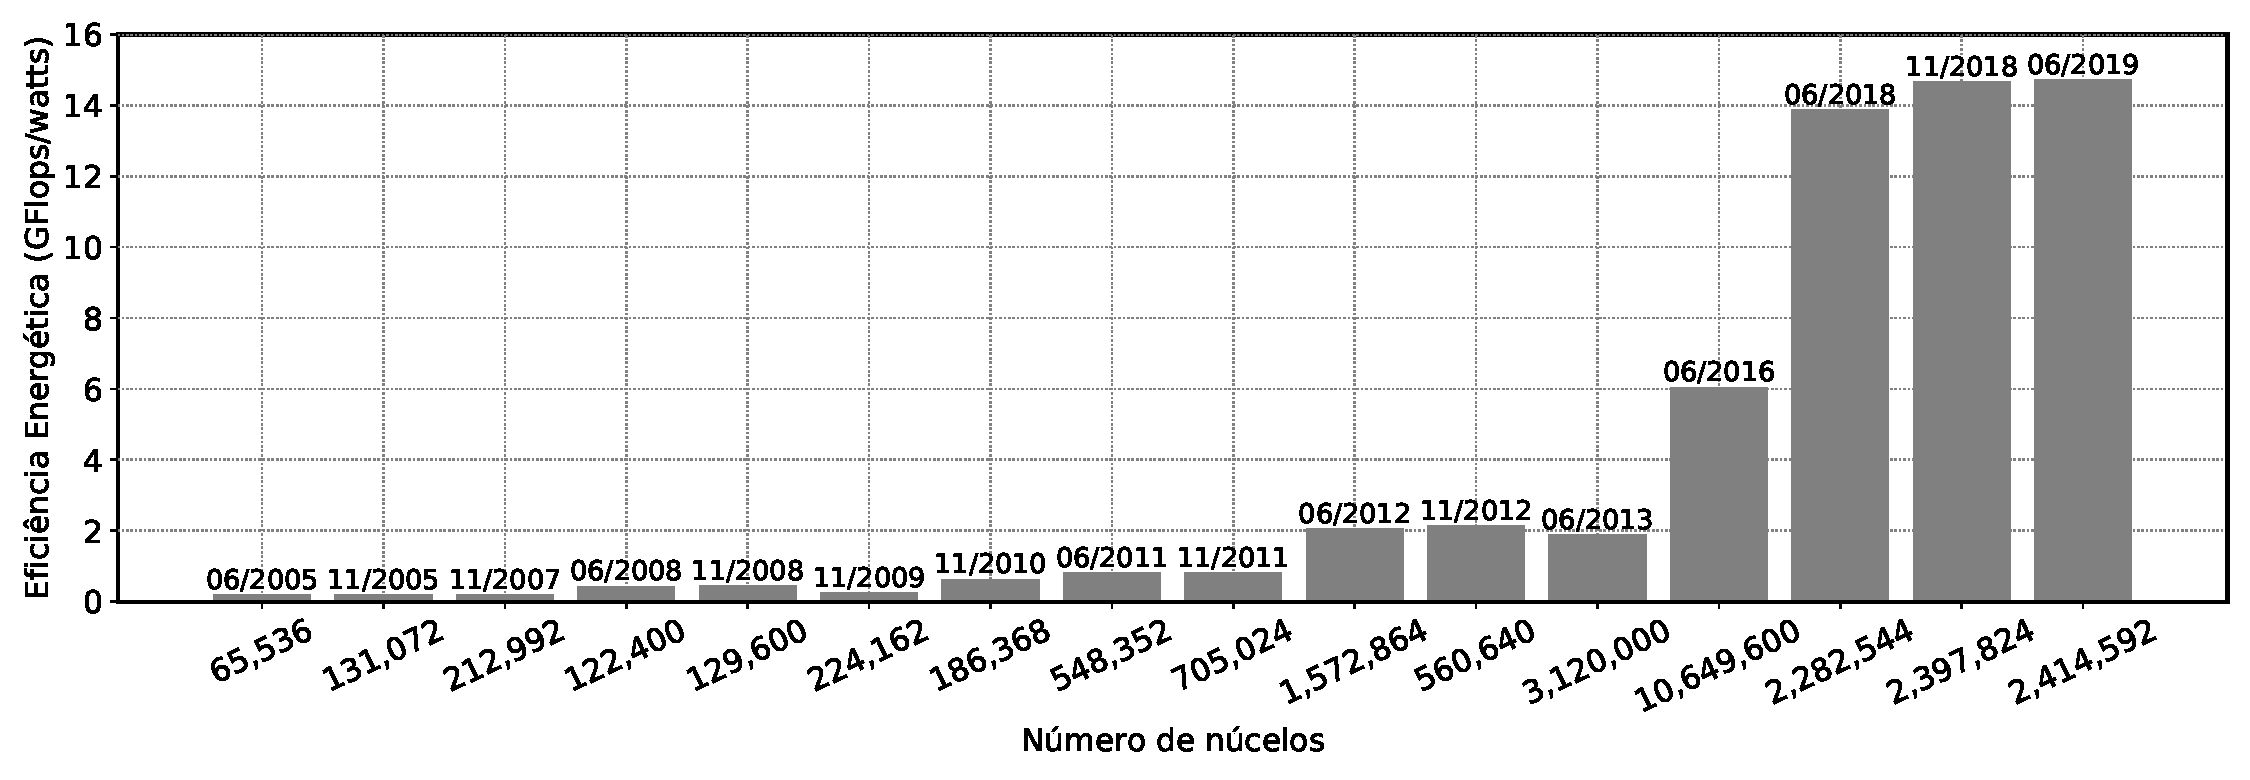
\includegraphics[width=1\linewidth, keepaspectratio]{Figure_Efficiency_X_Cores_Top500.pdf}
  \fonte{Gráfico desenvolvido pelo autor.}
\end{figure}

\begin{figure}[tb]
  \centering
  \caption{Evolução da eficiência energética do supercomputador número 1 do mundo segundo o \ranking TOP500.}
  \label{fig:eficienciaxyearstop500}
  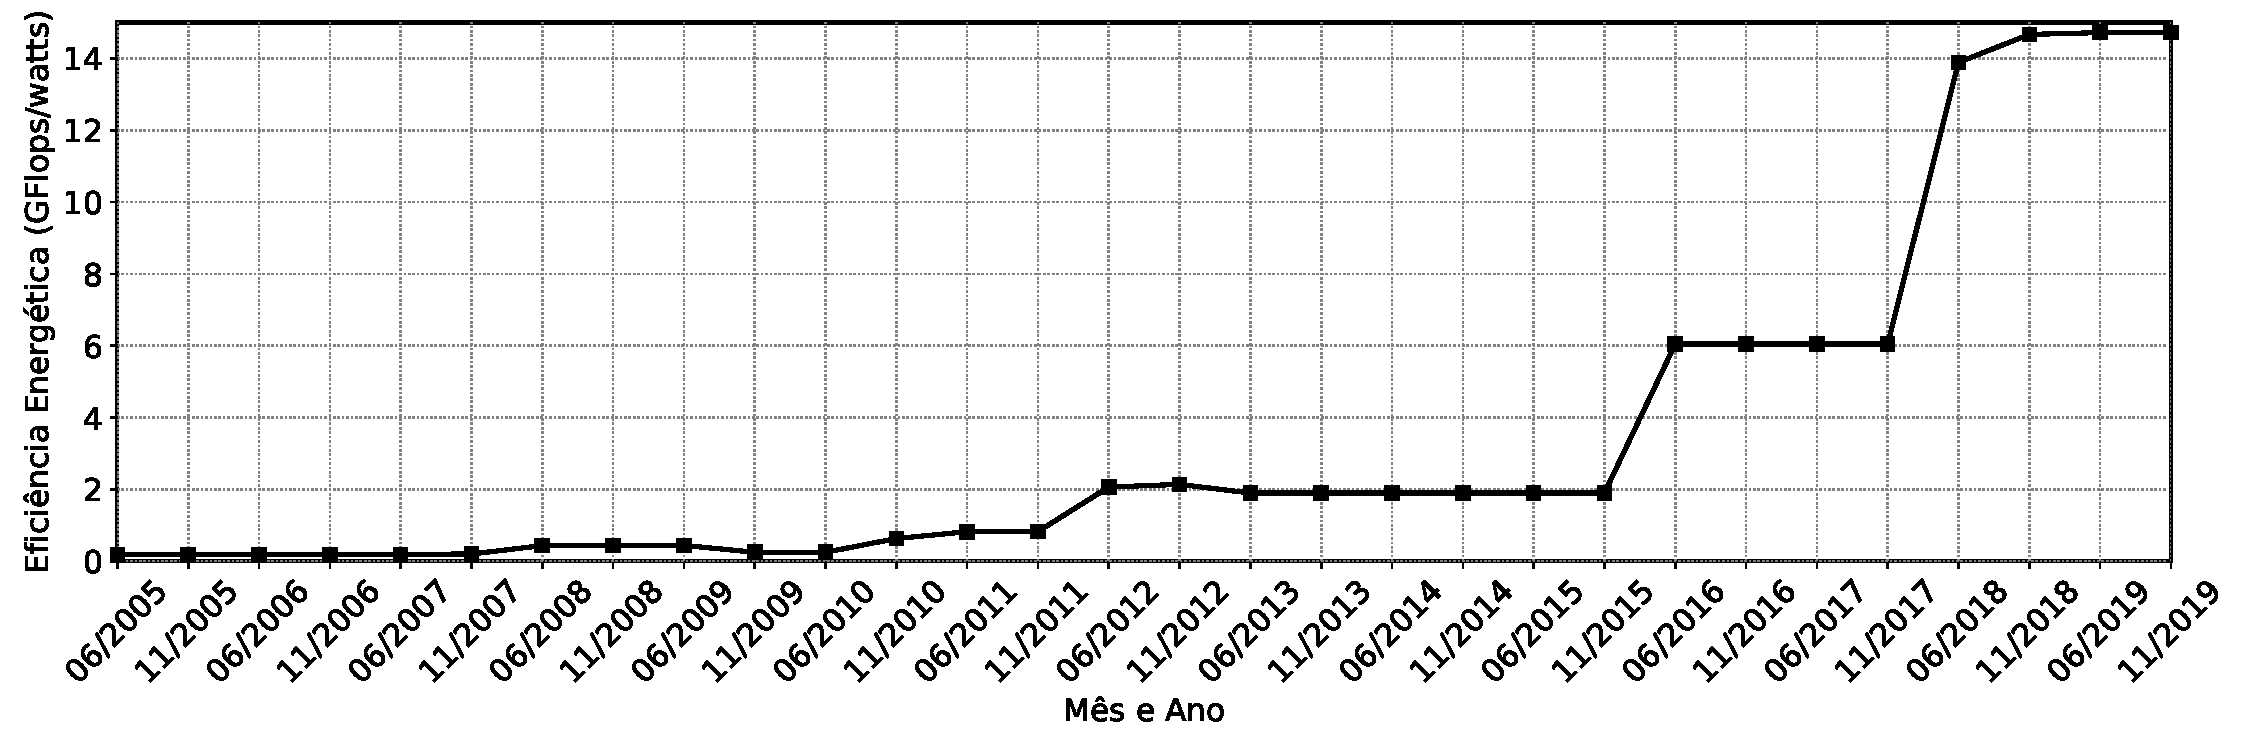
\includegraphics[width=1\linewidth, keepaspectratio]{Figure_Efficiency_X_Years_Top500.pdf}
  \fonte{Gráfico desenvolvido pelo autor.}
\end{figure}

Buscando novos tipos de arquiteturas paralelas que apresentem as características faltantes no problema de balanceamento apresentado acima, pesquisadores da área de \HPC realizaram diversos estudos voltados para essa questão, aplicando conceitos de \greencomputing \cite{greencomputingacm} no decorrer do desenvolvimento de suas soluções. Dentre estas soluções, temos o surgimento da classe de processadores \manycore de baixa potência, como o \mppa \cite{mppa2562013}, objeto de estudo deste trabalho, o Adapteva Epiphany \cite{olofsson2014}, e o SW26010, utilizado no atual terceiro supercomputador mais poderoso do mundo, o \textit{Sunway TaihuLight} \cite{fu2016sunway}. Vale citar que o SW26010 desbancou em 2016 o supercomputador que assumia, desde 2013, a primeira posição do \ranking TOP500, obtendo duas vezes mais desempenho que esse e reduzindo em três vezes o consumo energético, explicando também o ganho elevado em eficiência em ambas as Figuras \ref{fig:eficienciaxcorestop500} e \ref{fig:eficienciaxyearstop500} no mês de junho de 2016.

Para avaliar o desempenho e consumo energético do \mppa, \textit{Souza} \etal propuseram o desenvolvimento do \bench \capb, o qual, em sua primeira versão, utilizava uma \API de comunicação síncrona entre processos denominada \IPC \cite{mppa2562013}. Essa \API possui algumas deficiências, como o baixo nível de abstração, requerendo conhecimento prévio da arquitetura alvo para implementações paralelas eficientes, e a realização de sincronizações implícitas muitas vezes não necessárias nas operações de envio e recebimento de dados, o que leva a queda de desempenho da aplicação. Ao realizar a otimização do \bench, \textit{David} \etal o portaram com a \ASYNC, uma \API com maior nível de abstração e com conceitos de assincronismo, aumentando o potencial de desempenho da aplicação. Além disso, alterações na implementação de todas as aplicações foram realizadas de modo a otimizá-las ainda mais.

Portanto, para realizar uma comparação justa entre as \APIs citadas acima, faz-se necessário atualizar a lógica de implementação das aplicações da versão antiga do \bench, para que essas se equivalham às novas implementações, criando assim um ambiente propício para comparar aspectos puramente das tecnologias de comunicação citadas, utilizando as duas versões do \bench para isso. A comparação entre ambas as implementações será responsável por determinar qual \API se comporta de maneira mais robusta no \mppa em certos contextos, onde os dados acerca do tempo de execução, quantidade de dados enviados e recebidos e gasto energético de cada aplicação serão as métricas para essa determinação. Assim, teremos dados de execução das duas \APIs numa mesma versão de placa do \mppa, resultando numa base de dados concreta para a tomada de decisão sobre qual das duas \APIs escolher na hora de implementar uma nova aplicação.

\section{Objetivos}
\label{sec:objetivos}

Com base no que foi exposto, são apresentados abaixo o objetivo geral e os objetivos específicos deste trabalho.

\subsection{Objetivo Geral}
\label{sec:objetivogeral}

O objetivo deste trabalho é obter dados concretos acerca da execução de aplicações de diversos domínios de problemas no \mppa, utilizando as duas \APIs já citadas e o \capb, podendo assim comparar as execuções de cada aplicação em cada cenário específico possível dentro do processador, obtendo identificadores precisos que, em momentos futuros, possam apontar qual das duas \APIs utilizar, dependendo do domínio de problema de uma certa aplicação.

\subsection{Objetivos Específicos}
\label{sec:objetivosespecifico}

\begin{itemize}
\item Investigar a viabilidade do uso do \mppa para a área de \HPC.
\item Estudar aspectos das \APIs de comunicação existentes no \mppa, mais especificamente, a \ASYNC e a \IPC.
\item Avaliar os custos e benefícios do \mppa em relação ao desempenho e gasto energético, assim como sua utilidade para a Computação Sustentável (\greencomputing)
\item Comparar as \APIs \ASYNC e \IPC a fim de prover métricas precisas para a escolha de uma das duas numa futura implementação.
\end{itemize}

\section{Contribuições do trabalho}

Este trabalho é continuação de um projeto de iniciação científica desenvolvido por \textit{David} \etal, o qual resultou em um resumo expandido publicado na Escola Regional de Alto Desempenho da Região Sul no ano de 2019:

\begin{itemize}
  \item ORDINE, D. G. V.; PODESTA JUNIOR, E. ; PENNA, P. H. ; CASTRO, M. \textbf{Otimização de Aplicações do CAP Bench para o Processador \mppa.} In: Escola Regional de Alto Desempenho da Região Sul (ERAD/RS), 2019, Três de Maio. Anais da Escola Regional de Alto Desempenho da Região Sul (ERAD/RS). Porto Alegre: Sociedade Brasileira de Computação (SBC), 2019.
\end{itemize}

\section{Organização do trabalho}

Este trabalho está dividido da seguinte forma. O Capítulo \ref{ch:fundamentacaoteorica} mostra os conceitos teóricos que foram utilizados para a produção dessa dissertação. O Capítulo \ref{ch:trabcorrelatos} apresenta alguns trabalhos relacionados a este. O Capítulo \ref{ch:desenvolvimento} contém toda a proposta deste projeto, detalhando tudo que foi feito, assim como explicando as métricas que serão expostas nos resultados. O Capítulo \ref{ch:resultados} apresenta os resultados preliminares já obtidos. Para finalizar, o Capítulo \ref{ch:conclusao} conclui este trabalho.

\chapter{Fundamentação Teórica}
\label{ch:fundamentacaoteorica}

Neste capítulo são apresentados conceitos relacionados a Computação Paralela, por exemplo, padrões arquiteturais, na Seção \ref{sec:arquiteturasparalelas}, e tecnologias de programação, na Seção \ref{sec:bibliotecasdevparalelo}. Também são mostrados algumas características do \mppa na Seção \ref{sec:mppa256}.

\section{Arquiteturas Paralelas}
\label{sec:arquiteturasparalelas}

Existem três tipos de sistemas com múltiplos processadores, segundo \textit{Tanenbaum} \etal : os multiprocessadores, os multicomputadores e os sistemas distribuídos \cite{TanenbaumMordenOS}. São detalhados nesta seção conceitos acerca das arquiteturas multiprocessadores e multicomputadores.

\subsection{Multiprocessadores}
\label{sec:multiprocessadores}

A principal característica de uma arquitetura multiprocessador é o acesso compartilhado ao barramento de memória do sistema, a \RAM, por diversas \CPUs. Programas executando em qualquer um dessas \CPUs possuem espaços de endereçamento físicos únicos na \RAM e as \threads de um desses programas fazem uso de um mesmo espaço de memória, através de operações de escrita e leitura, para se comunicarem. Um fato peculiar dessa arquitetura é a possibilidade de ocorrer problemas de concorrência quando duas ou mais \threads de um mesmo programa executam em diferentes \CPUs, onde, na visão de uma \CPU, ela escreve um valor em uma posição de memória e lê outro valor daquela mesma posição, pois uma \thread executando em outra \CPU alterou o valor daquela posição. 

Multiprocessadores são também classificados em dois tipos, de acordo com a velocidade de acesso a uma posição de memória. Quando uma certa palavra na memória pode ser lida na mesma velocidade que qualquer outra, são chamados de multiprocessadores com acesso uniforme a memória - \UMA. Já quando a velocidade de leitura em diferentes posições de memória muda, são chamados de multiprocessadores com acesso não uniforme a memória - \NUMA. 

A arquitetura mais simples de um multiprocessador \UMA, exemplificada na Figura \ref{fig:umasimples}, envolve um único barramento conectando duas ou mais \CPUs a um módulo de memória, permitindo que todas as \CPUs realizem operações de leitura e escrita neste módulo. Quando uma \CPU necessita ler alguma palavra da memória, primeiramente ela verifica se o barramento está ocupado. Caso não, informa à memória, através do barramento, qual endereço deseja obter o valor, aguardando o recebimento deste pelo mesmo barramento. Caso esteja, a \CPU aguarda a liberação do barramento. Para uma pequena quantidade de \CPUs, o tempo de espera médio para o acesso ao barramento tende a ser pequeno e tolerável. Porém, quando elevam-se em algumas dezenas o número de \CPUs observa-se o principal problema deste exemplo de arquitetura \UMA: a ociosidade, por muito tempo, de grande parte das \CPUs, enquanto aguardam pelo acesso ao barramento.



\begin{figure}[tb]
  \centering
  \caption{Diferentes esquemas possiveis de um multiprocessador UMA baseado em barramento.}
  \subcaptionminipage[fig:umasimples]%
    {.4\linewidth}%
    {Sem \textit{cache}}%
    {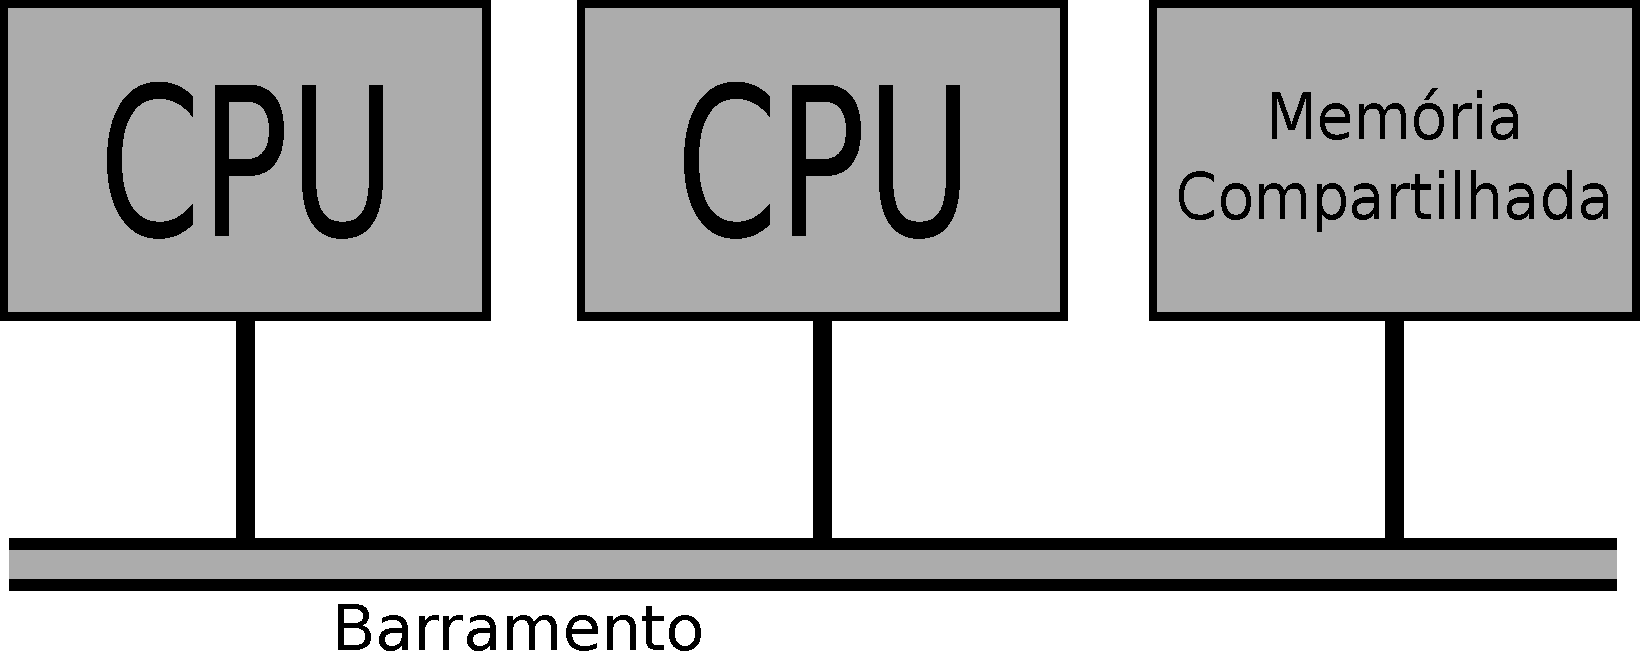
\includegraphics[width=.9\linewidth]{umasimples.pdf}}%
  \hfill% 
  \subcaptionminipage[fig:umacomcache]%
    {.4\linewidth}%
    {Com \textit{cache}}%
    {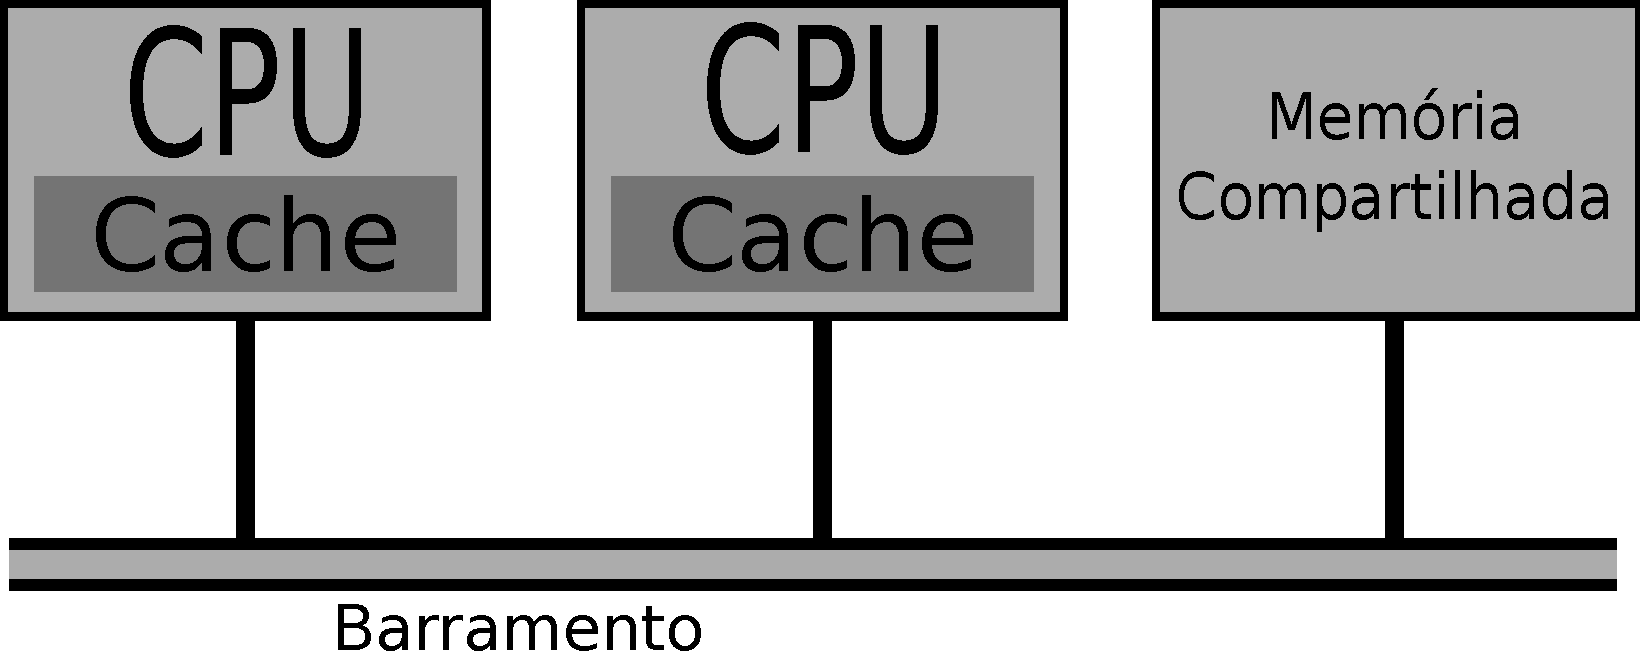
\includegraphics[width=.9\linewidth]{umacomcache.pdf}}%
  \hfill% 
  \subcaptionminipage[fig:umacomcacheememprivada]%
    {.4\linewidth}%
    {Com \textit{cache} e memórias privadas}%
    {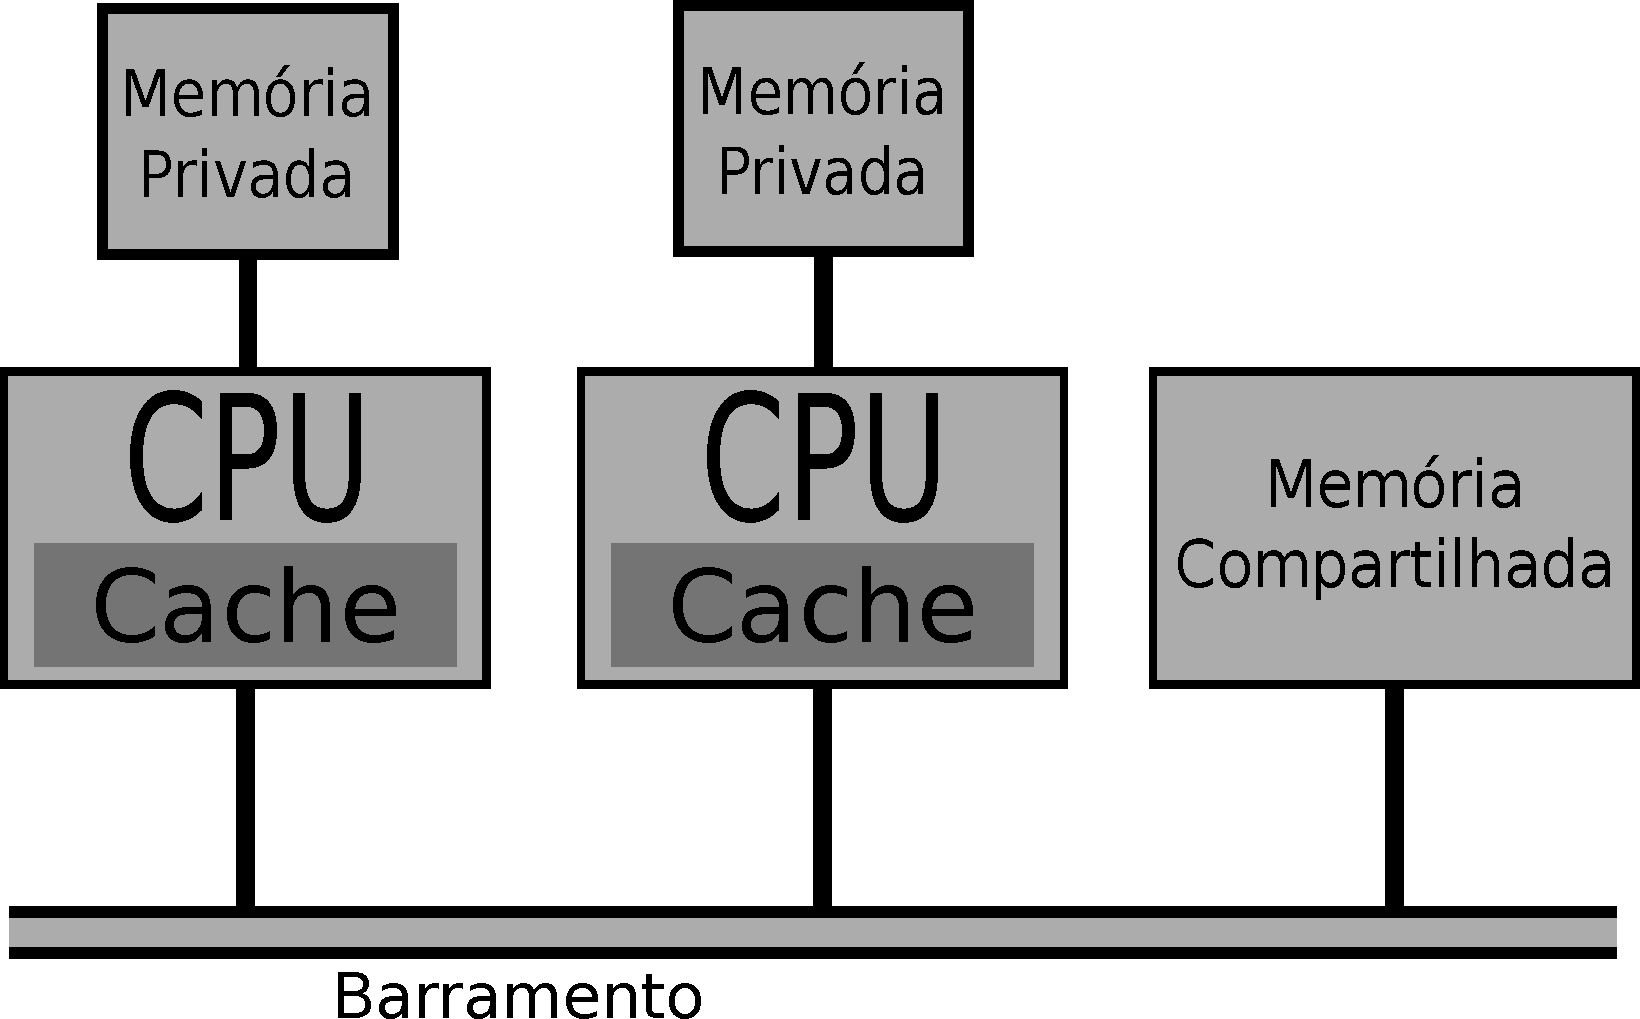
\includegraphics[width=.9\linewidth]{umacomcacheememprivada.pdf}}%
  \hfill% 
  \fonte{Imagens desenvolvidas pelo autor, adaptadas de \textit{Tanenbaum} \etal \cite{TanenbaumMordenOS}.}
\end{figure}

Adicionar \caches às \CPUs, como na Figura \ref{fig:umacomcache}, é uma solução para reduzir o gargalo imposto sobre o barramento, já que agora valores podem ser lidos diretamente da \cache local, a qual está muito mais próxima da \CPU e possui tempo de acesso muito menor. Outra possibilidade é adicionar, além das \caches, memórias privadas locais,  como na Figura \ref{fig:umacomcacheememprivada}. Compiladores podem colocar nessas memórias todos os dados que são somente de leitura, por exemplo, constantes, o código do programa, strings e pilhas, utilizando assim esta segunda configuração de forma otimizada. Ambas configurações removem grande parte do tráfego no barramento, tornando seu uso exclusivamente para as variáveis compartilhadas entre \threads.

A adição de \caches impõe uso de protocolos de coerência para que não haja inconsistência entre os valores de um mesmo endereço de memória nas diferentes \caches. Primeiramente, para otimizar as operações de leitura, quando uma palavra é referenciada, todo o bloco que contém essa palavra, geralmente de 32 ou 64 \bytes, é colocado na \cache. Já para garantir a coerência, cada bloco é marcado como sendo somente de leitura, podendo assim estar presente em outras \caches, ou de leitura e escrita, não devendo estar presente em nenhuma outra \cache neste caso. Quando uma \CPU tenta alterar um valor que está presente em outras \caches além de sua própria, o \hardware do barramento informa essa operação às outras \caches, as quais tratam esse contexto de duas formas. Caso o valor da \cache seja o mesmo em memória, podem simplesmente descartá-lo, buscando o novo valor na memória se necessário. Caso outra \cache tenha um valor diferente daquele em memória, é necessário ou salvá-lo na memória ou transferi-lo diretamente para a \cache que solicitou a operação de escrita.

Quando necessita-se de um número de processadores na ordem das centenas, a arquitetura \UMA acaba sendo inviável. Assim, introduz-se a arquitetura \NUMA, trazendo com ela a ideia de diferentes tempos de acesso para diferentes posições de memória. Multiprocessadores \NUMA provém essa escalabilidade implementando um espaço de endereçamento único para todas as \CPUs através de uma rede de interconexão, como na Figura \ref{fig:multiprocessadornuma}, o que causa a diferença nos tempos de acesso, os quais serão totalmente dependentes do local da memória que se deseja acessar um valor relativo ao local da \CPU que requisitou este acesso. Logo, outra propriedade desta arquitetura é o acesso mais rápido à memória local de um ou um conjunto de \CPUs, em comparação com o acesso à memória remota. Vale salientar que programas desenvolvidos para multiprocessadores \UMA conseguem ser executados em arquiteturas \NUMA, devido a ambas possuírem um espaço de endereçamento único. Porém, estes programas irão obter performance inferior, já que não foram otimizados para considerar as diferenças de tempo entre acesso à memória local e remota.

\begin{figure}[tb]
  \centering
  \caption{Esquema genérico de um multiprocessador NUMA.}
  \label{fig:multiprocessadornuma}
  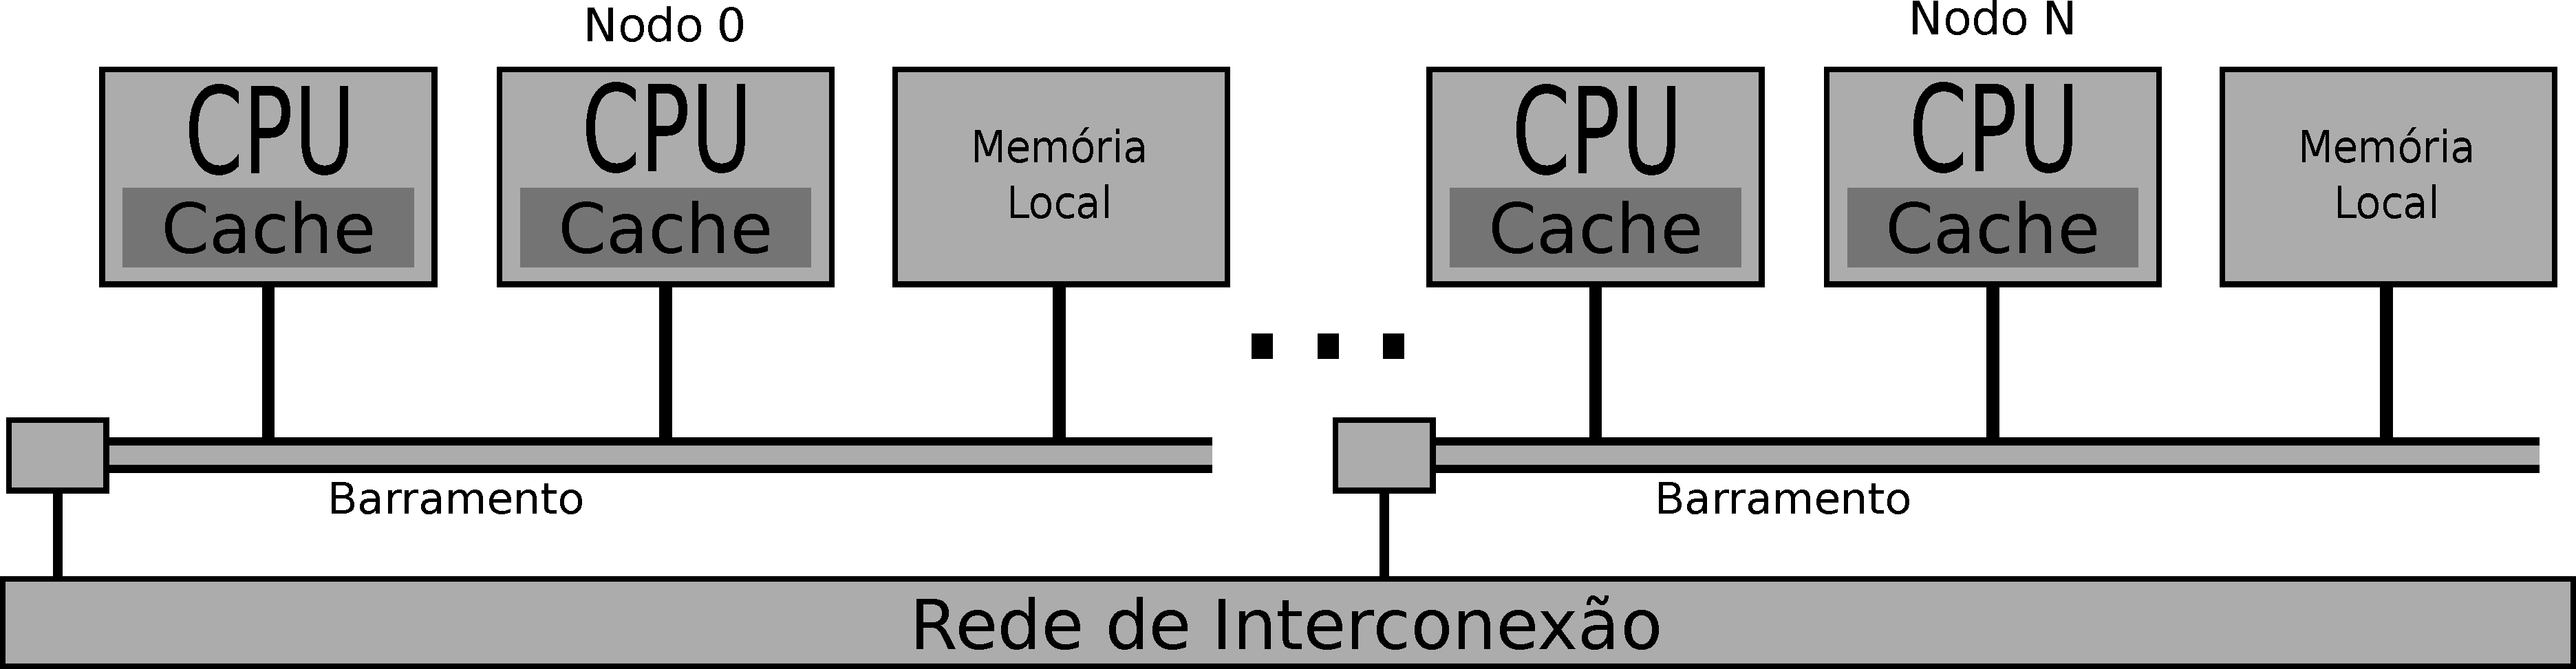
\includegraphics[width=.9\linewidth, keepaspectratio]{numa.pdf}
  \fonte{Imagem desenvolvida pelo autor, adaptada de \textit{Tanenbaum} \etal \cite{TanenbaumMordenOS}.}
\end{figure}

A medida que o tamanho de um \transistor diminui, o número de \transistors em um \chip tende a aumentar. Diversas soluções exploram o que fazer com este número crescente de \transistors, por exemplo, adicionar \caches poderosas de muitos \textit{mega}\bytes ou colocar duas ou mais \CPUs, também chamadas de núcleos (em inglês \textit{cores}), neste mesmo \chip. Em certo ponto, o aumento no tamanho da \cache traz pouquíssimo ganho em porcentagem de \textit{hit} (quantidade de vezes que é possível buscar um dado diretamente na \cache), mostrando assim que o investimento no paralelismo trazido pelos múltiplos núcleos como recurso para ganho em desempenho é uma opção a se considerar. Assim, \chips \multicore são uma mescla de múltiplas \CPUs com múltiplos níveis de \cache inseridos em um espaço muito menor que um multiprocessador, sendo por isso também chamados de \CMPs.

Apesar de serem parecidos, existem algumas diferenças entre os \CMPs e os multiprocessadores. Primeiramente, em muitos \CMPs ocorre o compartilhamento da \cache nível 2 ou 3 entre suas \CPUs, o que não acontece nos multiprocessadores, que possuem \caches totalmente privadas em todos os níveis. Além disso, a probabilidade de que falhas em componentes compartilhados levem a impossibilidades em múltiplas \CPUs ao mesmo tempo é muito maior nos \CMPs, devido a proximidade de conexão das \CPUs. Por fim, existem \chips \multicore em que todos os núcleos são feitos para atender a uma ampla gama de contextos, enquanto que em outros, além das \CPUs principais, existem também núcleos específicos para alguns problemas, como decodificação de áudio e vídeo ou interfaces de rede. 

Apesar de não haver uma barreira de distinção entre um \chip \manycore ou \multicore, pode-se chama-lo de \manycore quando a perda de um núcleo tem um pequeno impacto na performance total do \chip. Um problema com arquiteturas \manycore é a escalabilidade entre manter as \caches de todas as \CPUs coerentes e ainda assim elevar o desempenho ao elevar o número de núcleos. Cientistas da área de \HPC temem que essas duas variaveis não escalem proporcionalmente, tornando o custo de gerenciar essas \caches tão alto que a adição de um novo núcleo de pouco ajudara no aumento em performance. Este problema é também conhecido como a barreira de coerencia  (\textit{coherency wall}) \cite{TanenbaumMordenOS}.

Para o futuro dos \manycore, espera-se processadores que invistam mais  na comunicação entre \CPUs através da troca de mensagens extremamente rápidas via \hardware e através de uma memória compartilhada, deixando de lado parte da coerência de \cache. Uma \GPU é um dos exemplos mais comuns de um processador \manycore, possuindo milhares de pequenos núcleos especializados na rápida execução de cálculos e sem uma lógica complexa de \cache, ou seja, priorizam o processamento. Desta maneira, \GPUs são excepcionais para a execução paralela de pequenas tarefas, como a renderização de \textit{frames} para jogos. Programar para uma \GPU é uma tarefa difícil e muitas vezes algumas linguagens de programação especiais são utilizadas, como a OpenGL ou a CUDA, da NVIDIA. Essa dificuldade se dá, principalmente, pelo fato dos núcleos de uma \GPU executarem exatamente a mesma instrução em diferentes fatias de um dado, ou seja, pelo fato da \GPU ser uma máquina \SIMD.

\subsection{Multicomputadores}
\label{sec:multicomputadores}

Multicomputadores surgiram na dificuldade de aumentar o poder de processamento de um multiprocessador quando se atinge grandes escalas em relação ao número de núcleos. Ao contrário dos multiprocessadores, multicomputadores não compartilham memória, sendo relativamente fáceis de se construir, tendo como componente principal um computador com uma placa de rede de alta performance, sem mouse, teclado e monitor. Neste sistema, também chamado de \textit{Cluster Computers} ou {Cluster Of Workstations} (COWs), é necessário um \textit{design} inteligente da rede que irá conectar os computadores para que se possa obter um alto desempenho.

Um nó de um multicomputador consiste então em um computador, com uma \CPU, memória, placa de rede e um HD. Diversas são as topologias possíveis para a rede que conecta os nós, como mostrado na Figura \ref{fig:topologiamulticomputadores}. Sistemas pequenos utilizam-se de apenas um \textit{switch} para conectar os nós entre si, os quais são então organizados em forma de estrela, como na Figura \ref{fig:topologiamulticomputadores}(a). Também é possível organizar os nós em forma de anel, onde cada nó se conecta aos nós da sua esquerda e direita, como na Figura \ref{fig:topologiamulticomputadores}(b), eliminando a necessidade de um \textit{switch}. Porém, o problema dessas arquiteturas é a escalabilidade, a qual dificulta o ganho em desempenho a medida que se aumenta o número de nós devido ao tempo de viagem dos dados entre nós.

\begin{figure}[tb]
  \centering
  \caption{Tipos de topologias de rede de multicomputadores.}
  \label{fig:topologiamulticomputadores}
  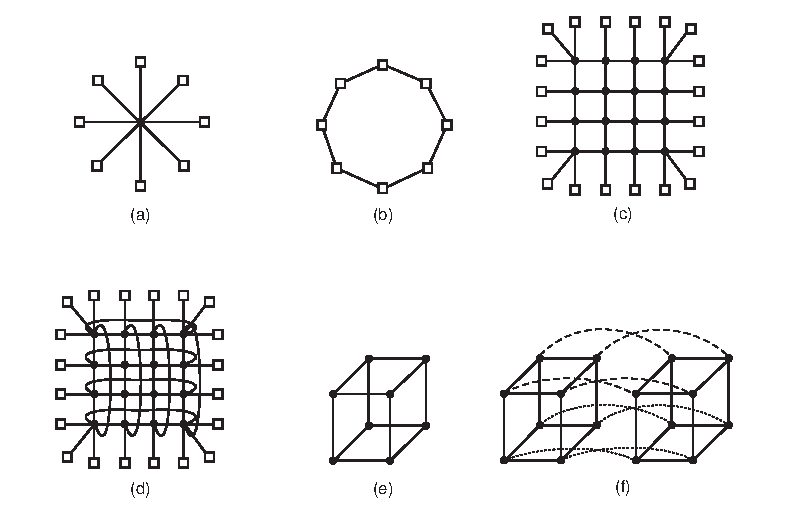
\includegraphics[width=.9\linewidth, keepaspectratio]{topologia.pdf}
  \fonte{\cite{TanenbaumMordenOS}.}
\end{figure}

Topologias mais complexas, como a malha (\textit{grid} ou \textit{mesh}), mostrada na Figura \ref{fig:topologiamulticomputadores}(c), ou a \textit{double torus}, mostrada na Figura \ref{fig:topologiamulticomputadores}(d), são mais escaláveis do que as apresentadas anteriormente. Nessas topologias, os nós são conectados em \textit{switches} e estes são conectados entre si, formando um \textit{layout} de malha no sistema. Dentre as duas citadas, a \textit{double torus} é mais escalável devido a conexão entre nós nas arestas da rede, trazendo assim conexões extras ao sistema, o que aumenta a tolerância a faltas e o desempenho, já que o caminho entre estes nós se torna menor. Este tipo de rede possui uma propriedade chamada de diâmetro, que é o caminho mais longo entre dois nós. Para topologias bidimensionais como a malha, o diâmetro aumenta proporcionalmente a raiz quadrada do número de nós. \textit{Layouts} \textit{n} dimensionais, como mostrado na Figura \ref{fig:topologiamulticomputadores}(e) (tridimensional) e na Figura \ref{fig:topologiamulticomputadores}(f) (quadrimensional), são ainda mais escaláveis, já que o diâmetro diminui à medida que se aumenta o número de dimensões da rede, tendo como única desvantagem o custo elevado, devido ao grande número de ligações presentes entre nós e \textit{switches}.

A comunicação entre processos rodando em diferentes \CPUs, num multicomputador, se dá através da troca de mensagens entre estes. Basicamente, o \SO presente no multicomputador é o responsável por realizar essa troca, através de funções acessíveis somente a ele. Porém, bibliotecas podem fornecer abstrações a essas funções, tornando a troca de mensagens também disponível para os processos usuário e as simplificando, visto que abstraem toda uma lista de invocações de funções em uma única função. Essa troca de mensagens pode ser reduzida a duas funções, chamadas de \textit{send} e \textit{receive}. A função \textit{send} é responsável por enviar uma mensagem de uma \CPU para outra, passando parâmetros como o destino da mensagem e o endereço onde aquela mensagem se encontra. Já a função \textit{receive} é responsável por receber a mensagem, tendo como parâmetros, por exemplo, o endereço de onde a mensagem será lida e o endereço onde será armazenada. Por fim, essas funções podem ser síncronas, bloqueando o processo que envia ou recebe a mensagem até que a operação seja concluída, ou assíncronas, não bloqueando o processo que realizou tal operação.

\section{\mppa}
\label{sec:mppa256}

\begin{figure}[tb]
  \centering
  \caption{Visão arquitetural simplificada do \mppa.}
  \label{fig:mppa256overview}
  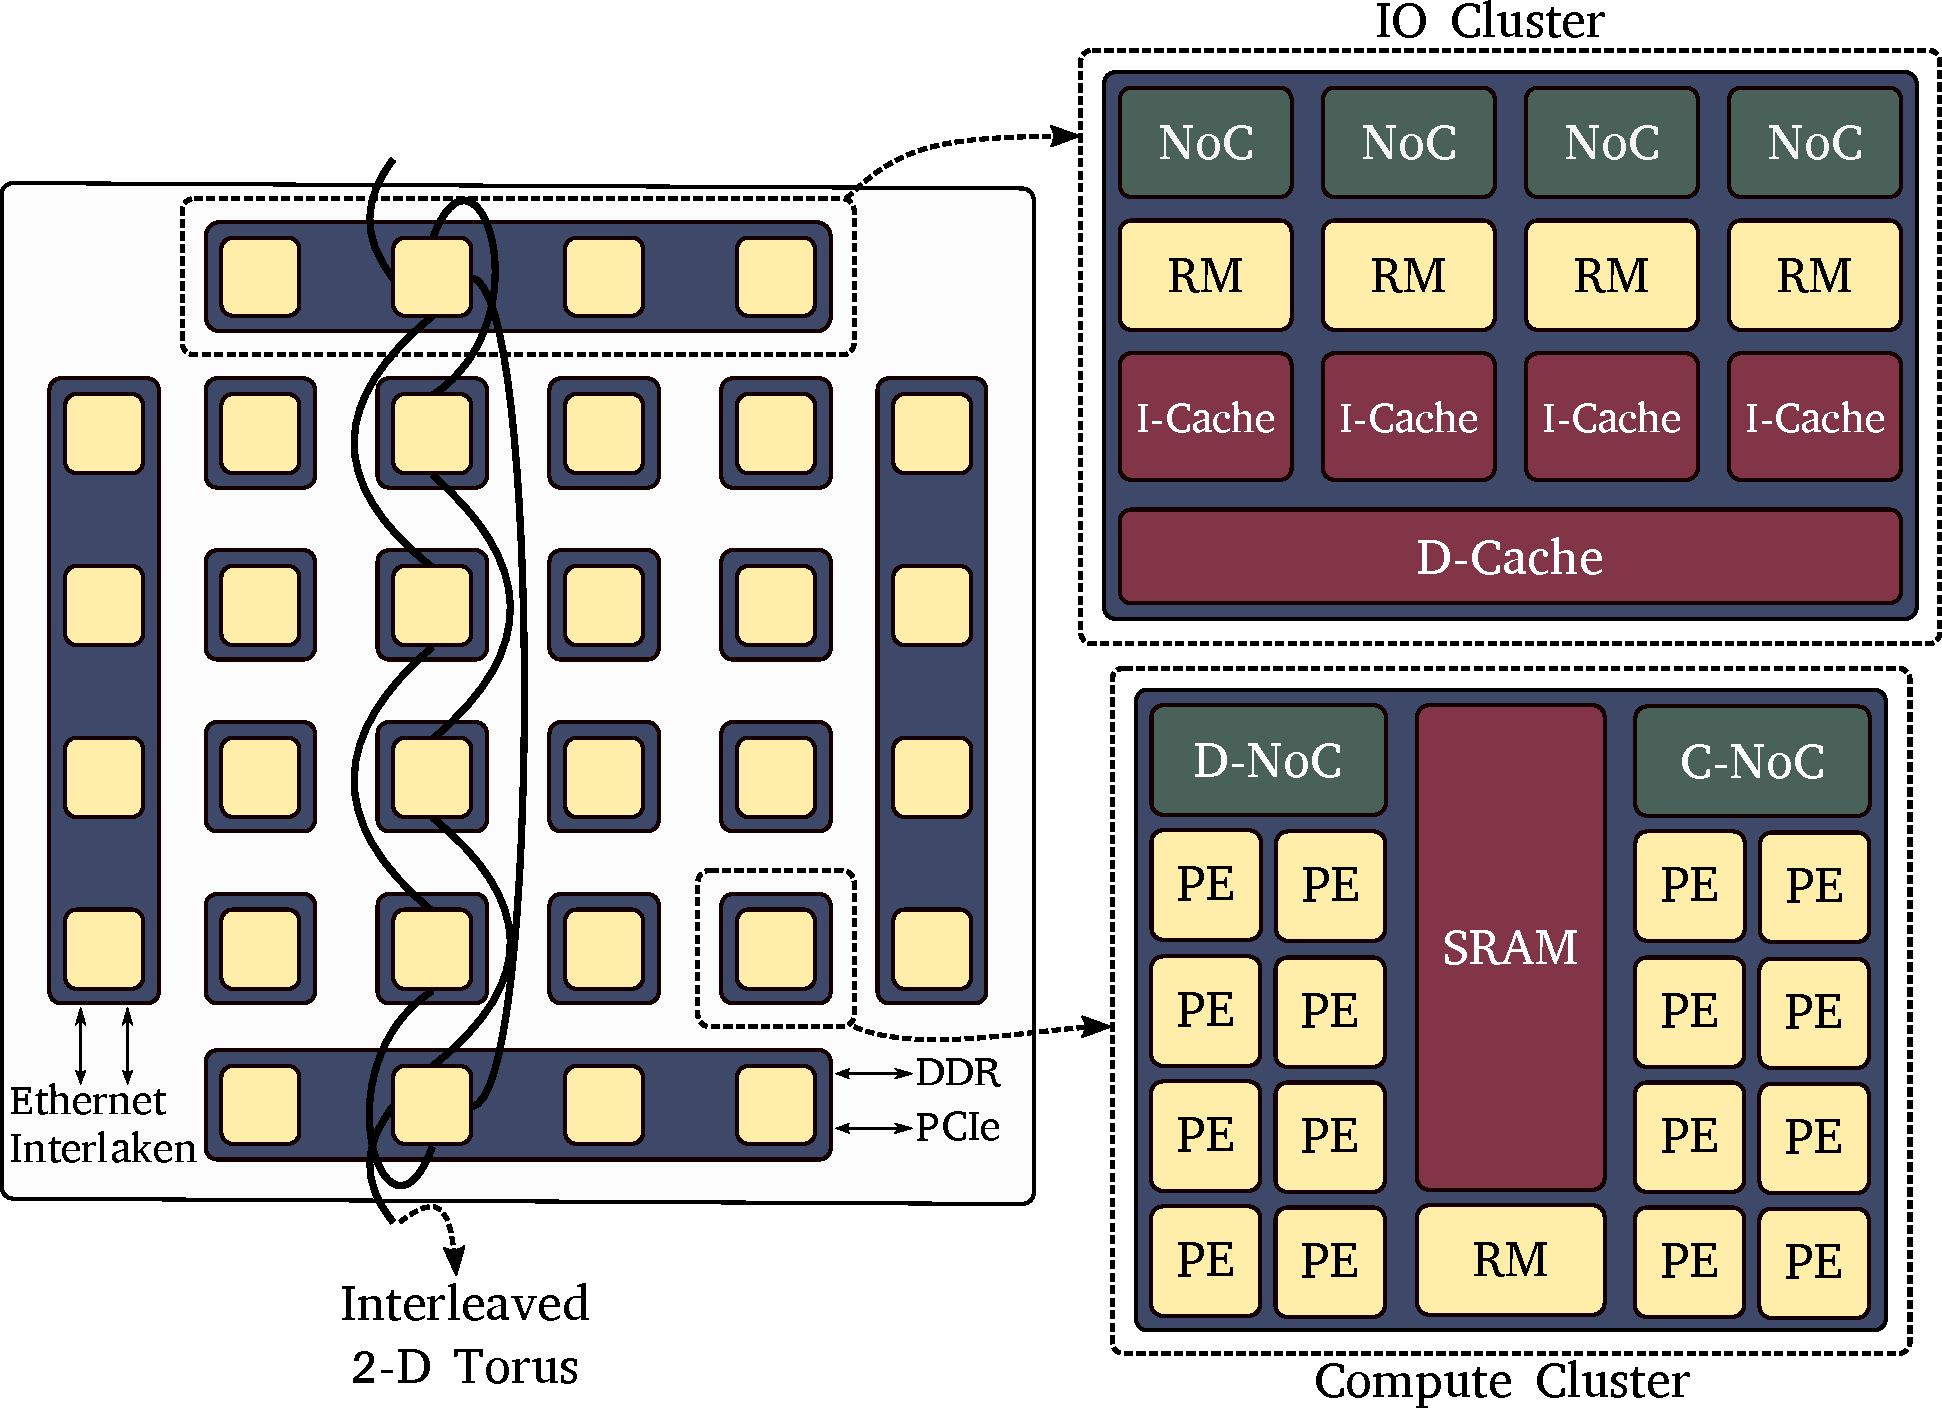
\includegraphics[width=.7\linewidth, keepaspectratio]{mppa-overview.pdf}
  \fonte{\cite{Penna2018OS}.}
\end{figure}

Desenvolvido pela empresa francesa Kalray, o \mppa é um processador de baixa potência que reflete o estado da arte dos \manycore. Uma visão geral do processador é mostrada na Figura \ref{fig:mppa256overview}. O \mppa possui 16 \CCs e 4 \textit{clusters} de \IO. Cada CC possui: \textbf{(i)} 16 núcleos para executar \textit{threads} de usuário em modo ininterrupto e não preemptivo, os quais atuam com frequência de 400 MHz; \textbf{(ii)} um gerenciador de recursos responsável por executar
o sistema operacional e gerenciar comunicações; \textbf{(iii)} uma memória compartilhada de 2MB, possibilitando alta largura de banda e taxa de transferência entre núcleos de um mesmo \textit{cluster}; e  \textbf{(iv)} dois controladores de Rede-em-Chip \textit{Network-on-Chip} -- NoC), um para dados e outro para controle. Cada núcleo possui duas memórias \cache, uma para dados e outra para instruções. As \caches são associativas \textit{2-way} privadas e possuem 32kB \cite{Podesta2018Stencil}.

Por outro lado, \textit{clusters} de \IO realizam comunicações com dispositivos externos, onde dois destes apresentam acesso às memórias externas \textit{Low-Power Double Data Rate 3 (LPDDR3)} de 2GB. É importante salientar que um \CC não pode acessar diretamente os dados da memória de outros \textit{clusters}. Logo, o processador apresenta um modelo de memória distribuído \cite{Castro-Souza-CCPE:2016, Podesta2018Stencil}.

\section{Desenvolvimento de Aplicações Paralelas}
\label{sec:bibliotecasdevparalelo}

Durante o domínio de processadores \singlecore no mercado, para que uma aplicação ganhasse aumento em performance, bastava esta ser executada em um processador com maior frequência de \textit{clock}. Isso removia parte da responsabilidade do desenvolvedor em implementar melhorias na aplicação, já que bastava o \textit{upgrade} no hardware para obter essas melhorias. Nestes processadores, instruções são executadas de forma sequencial em um único núcleo. Já em processadores \multicore e \manycore, existem múltiplos núcleos executando diferentes instruções, possivelmente, de diferentes programas. Essa divisão de tarefas pode levar a diversos novos problemas, como \textit{deadlock} ou condições de corrida.

Diversas \APIs voltadas a programação paralela foram criadas para simplificar tanto a solução desses problemas como o desenvolvimento de aplicações que implementam paralelismo. Abaixo serão apresentadas duas das mais conhecidas \APIs para multiplataformas, a \OpenMP e o \MPI, assim como duas \APIs específicas para o \mppa, a \ASYNC e a \IPC.

\subsection{Bibliotecas multiplataforma}
\label{sec:bibliotecasmultiplataforma}

\subsubsection{Open Multi-Processing}
\label{sec:openmp}

A \OpenMP é uma das bibliotecas mais utilizadas para implementação de aplicações paralelas nas linguagens C, C++ e Fortran. Sua fama vem, principalmente, da abstração que a \API fornece, sendo possível ser utilizada em inúmeras plataformas. Por ser uma \API voltada ao \textit{multithreading}, utiliza-se do compartilhamento de memória entre as \threads de um mesmo programa para criar beneficios ao desenvolvedor, como variáveis de ambiente.

Esta biblioteca é centrada no modelo \textit{fork-join} (Figura \ref{fig:forkjoin}), onde, em determinados momentos do fluxo de execução de uma aplicação, temos a \thread principal instanciando outras \threads através de diretivas de compilação fornecidas pela própria \API, as quais serão executadas de forma independente, paralelamente ou concorrentemente entre si. A \thread principal também realiza uma sincronização com as \threads criadas através de uma barreira implícita, aguardando o término de todas as \threads para continuar com a execução. A criação de novas \threads se dá ao atingir uma região paralela, definida por algumas diretivas de compilação, como \texttt{\#pragma omp parallel for}, que paraleliza a execução de um \textit{loop} entre múltiplas threads. O código \ref{lst:parallelloop} produz, de forma paralela, um array com 10 posições, onde cada posição armazena um inteiro igual ao índice daquela posição.


\begin{figure}[tb]
  \centering
  \caption{Esquema do modelo \textit{fork-join}.}
  \label{fig:forkjoin}
  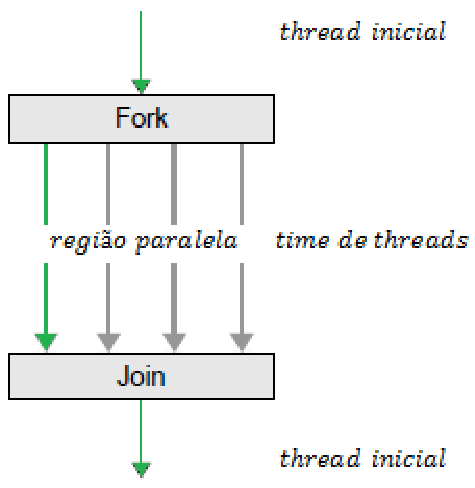
\includegraphics[width=.4\linewidth, keepaspectratio]{forkjoin.pdf}
  \fonte{\cite{forkjoinarticle}.}
\end{figure}

\begin{listing}[tb]
\caption{Execução de um \textit{loop} de forma paralela.}
\label{lst:parallelloop}
\begin{minted}[highlightlines={6}]{c}
    static void createArray() {
      int array[max];
      int index;
      int index_max = 10;

      #pragma omp parallel for
      for (index = 0; i < index_max; index++)
          array[index] = index;
    }
\end{minted}
\fonte{o autor.}
\end{listing}

As diretivas \texttt{private, default e reduction} permitem, na sequência, definir quais variáveis terão escopo privado, qual será o escopo padrão das variáveis, e qual variável será feito uma redução sobre e qual será o tipo de redução (reduções são operações primitivas seguras sobre uma variável compartilhada entre múltiplas \threads). O código \ref{lst:reductionloop} é parte de uma das aplicações do \capb, a \textit{Friendly Numbers}, e utiliza essas três diretivas para realizar uma contagem paralela, a qual será armazenada na variável \texttt{partial\_friendly\_sum}. Ambas implementações mostram que, com a adição de uma única linha, muda-se completamente o fluxo de execução do programa, sendo esta a maior vantagem da \OpenMP.

\begin{listing}[tb]
\caption{Leitura e armazenamento seguro em variável compartilhada entre \threads.}
\label{lst:reductionloop}
\begin{minted}[highlightlines={6}]{c}
  static int partial_friendly_sum = 0;
  ...
  static void countFriends() {
    int i; /* Loop indexes. */

    #pragma omp parallel for private(i) default(shared) reduction(+: partial_friendly_sum)
    for (i = offset; i < offset + tasksize; i++) {
      for (int j = 0; j < i; j++) {
        if ((allTasks[i].num == allTasks[j].num) && (allTasks[i].den == allTasks[j].den))
          partial_friendly_sum++;
      }
    }
  }
\end{minted}
\fonte{o autor.}
\end{listing}

Também pode-se definir qual será o nível de trabalho de cada \thread com a diretiva \texttt{schedule}. Através desta diretiva, definem-se três tipos de escalonamentos para as \threads: \texttt{static}, \texttt{dynamic} e \texttt{guided}. Com o \texttt{static}, todas as \threads irão receber a mesma quantidade de trabalho, sendo este o escalonamento padrão. Já a diretiva \texttt{dynamic} é utilizada quando as iterações podem ter uma grande diferença no seu tempo de execução, realizando uma atribuição dinâmica de tarefas, onde cada \thread recebe uma nova tarefa ao terminar a iteração atual. Por fim, \texttt{guided} é similar ao \texttt{dynamic}, porém, a \thread começa recebendo um grande número de iterações, e se adaptando conforme executa, recebendo mais ou menos iterações, dependendo do tempo que leva para executá-las.

\subsubsection{Message Passing Interface}
\label{sec:mpi}

\begin{listing}[tb]
\caption{Exemplo de uma aplicação usando \MPI.}
\label{lst:programmpi}
\begin{minted}[highlightlines={11,16,19}]{c}
  int main(int argc, char **argv) {
    int rank, size;

    MPI_Init(argc, argv);
    MPI_Comm_rank(MPI_COMM_WORLD, &rank);
    MPI_Comm_size(MPI_COMM_WORLD, &size);

    char mensagem_bcast[25] = "Transmitindo um broadcast";
    char mensagem_bcast_recebido[18];

    MPI_Bcast(&mensagem_bcast, 25, MPI_CHAR, 0, MPI_COMM_WORLD);

    if (rank > 0) {
      mensagem_bcast_recebido[18] = "Broadcast recebido";

      MPI_Send (&mensagem_bcast_recebido, 18, MPI_CHAR, 0, 0, MPI_COMM_WORLD);
    } else if (rank == 0) {
      for (int i = 1; i < size; i++) {
        MPI_Recv(&mensagem_bcast_recebido, 18, MPI_CHAR, i, MPI_ANY_TAG, MPI_COMM_WORLD, MPI_STATUS_IGNORE);
      }
    }

    MPI_Finalize();
    return 0;
  }
\end{minted}
\fonte{o autor.}
\end{listing}

Diferentemente da \OpenMP, o \MPI é baseada no modelo \SPMD, onde um mesmo programa é executado por diferentes processos, cada qual tendo acesso a uma determinada região de memória. Assim, o \MPI é usada em supercomputadores para abstrair a difícil tarefa de implementar nestes o paralelismo através da troca de mensagens entre processos em baixo nível. Com esta \API de alto nível, implementar o envio e recebimento de mensagens torna-se algo tão simples como chamar uma função, já que o \MPI abstrai diversas etapas em uma única função. A \API também adiciona identificadores únicos e um grupo de comunicação para cada processo, os quais são usados como parâmetros em diversas de suas funções. Além disso, determinadas funções podem ser executadas de forma síncrona ou assíncrona, aumentando o desempenho da aplicação.

Um fluxo simples de implementação utilizando o \MPI começa com a função \texttt{MPI\_Init()}, que inicia o ambiente de execução \MPI. Na sequência, obtém-se o \textit{id} de um processo através da função \texttt{MPI\_Comm\_rank()}, a qual recebe um comunicador, geralmente o comunicador padrão \texttt{MPI\_COMM\_WORLD}, como primeiro parâmetro e o endereço da variável que será armazenado o \textit{id} do processo como segundo. Também é possível obter o número máximo de processos em um grupo de comunicação através da função \texttt{MPI\_Comm\_size()}, a qual recebe no primeiro parâmetro um comunicador e no segundo o endereço da variável em que será armazenado este número. Além disso, existem as funções de envio e recebimento de mensagens, \texttt{MPI\_Send()} e \textttt{MPI\_Recv()}, as quais ambas recebem parâmetros como o buffer de dados sobre o qual será realizado a leitura ou armazenamento da mensagem, a quantidade de dados, o tipo do dado e o \textit{id} do processo que realizará o envio ou recebimento da mensagem, além de alguns parâmetros adicionais. Por fim, a função \texttt{MPI\_Finalize()} termina a execução do ambiente \MPI.

Ao contrário das funções \textttt{MPI\_Recv()} e \texttt{MPI\_Send()}, que são voltadas para comunicação entre dois processos, funções como \texttt{MPI\_Bcast()} e \texttt{MPI\_Barrier()} são feitas para que haja comunicação entre um grupo de processos. Com a \texttt{MPI\_Bcast()} define-se o envio de uma mensagem de um processo para todos os outros processos associados a um grupo de comunicação. Já com a \texttt{MPI\_Barrier()} cria-se uma barreira, onde um certo processo, ao chegar nesta barreira, aguarda todos os outros processos de um grupo de comunicação chegarem nela antes de continuar sua execução.

O código \ref{lst:programmpi} mostra um exemplo de implementação simples usando o \MPI. Neste exemplo, na linha 11 o processo com \textit{id} igual a 0 envia um \textit{broadcast} para todos os outros processos, os quais respondem na linha 16 ao processo de \textit{id} 0, que recebe esta resposta na linha 19. Assim, as linhas 18-20 são executadas somente pelo processo com \textit{id} igual a 0, enquanto que as linhas 14-16 são executadas por processos com \textit{id} maior que 0. 

\subsection{Bibliotecas específicas para o \mppa}
\label{sec:bibliotecasespecificasmppa}

\chapter{Trabalhos Correlatos}
\label{ch:trabcorrelatos}


\section{Benchmarks Voltados para HPC}
\label{sec:benchprahpc}

\section{Benchmarks Específicos para Manycores}
\label{sec:benchpramanycores}

\chapter{Desenvolvimento}
\label{ch:desenvolvimento}

\chapter{Resultados}
\label{ch:resultados}

\chapter{Conclusão}
\label{ch:conclusao}

\index{bobagem} Primeiro parágrafo da seção com uma frase sem sentido que só serve para ocasionar uma quebra e de demonstrar a configuração de indentação da primeira linha. Essa frase está aqui pois parágrafos de uma linha são feios.

Resultado do uso de siglas:
\begin{itemize}
\item Sigla que nunca expande: \API;
\item Sigla normal, expande no primeiro uso: \DHT, mas não no segundo: \DHT;
\item Siglas com plurais automaticos: \APIs e \DHTs;
\item Plural não-trivial: \SQs;
\item Forçando uma expansão (e no plural) \Glsfirstplural{DHT};
\item Usando uma sigla cujo comando é diferente da sigla: \WTC.
\end{itemize}

Resultado do glossário:
\begin{itemize}
\item Dois termos, \polling e \proxy;
\item Plural: \proxys.
\end{itemize}

Resultado de \mla|index|: primeiro um link normal \indexterm{tomate}, depois um capitalizado \indexTerm{tomate}.

\begin{defn}
  Exemplo de definição
\end{defn}

\begin{theorem}
  Exemplo de teorema
\end{theorem}

\begin{theoremproof}
  Exemplo de prova \qed
\end{theoremproof}

(Sub)enumerações e citações (verificar se OK com o idioma):
\begin{enumerate}
\item \cite{turing1937}:
  \begin{enumerate}
  \item \citeonline{turing1937}:
    \begin{enumerate}
    \item \citeonline{dijkstra1968};
    \end{enumerate}
  \end{enumerate}
\item \cite{turing1937,dijkstra1968};
\item \citeonline{turing1937,dijkstra1968}.
\end{enumerate}


\begin{listing}[tb]
\caption{Meta informações do presente documento.}
\label{lst:meta}
\begin{minted}[highlightlines={1,4-5}]{latex}
\titulo{Template \LaTeX{} para testes e dissertações do LAPESD/UFSC}
\autor{Omar Ravenhurst}
\data{1 de agosto de 2019} % ou \today
\tese % ou \dissertacao
\titulode{Doutor em Ciência da Computação}
\orientador{Prof. Ben Trovato, Dr.}
\coorientador{Prof. Lars Thørväld, Dr.}

\membrobanca{Prof. Valerie Béranger, Dr.}{Universidade Federal de Santa Catarina}
\membrobanca{Prof. Mordecai Malignatus, Dr.}{Universidade Federal de Santa Catarina}
\membrobanca{Prof. Huifen Chan, Dr.}{Universidade Federal de Santa Catarina}
\coordenador{Prof. Charles Palmer, Dr.}
\end{minted}
\fonte{o autor.}
\end{listing}


Resultado de \mla|\autoref|s:
\begin{itemize}
\item \autoref{lst:meta};
\item \autoref{alg:algoritmo};
\item \autoref{fig:figura} tem subfiguras:
  \begin{itemize}
  \item \autoref{fig:svg}
  \item \autoref{fig:brasao}
  \end{itemize}
\item \autoref{tb:tabela};
\item \autoref{ch:exemplo};
\item \autoref{sec:frutas};
\item \autoref{sec:goiaba};
\item \autoref{sec:jabuticaba};
\item \autoref{sec:tomate}.
\end{itemize}


\begin{algorithm}
  \caption{Exemplo do ambiente \texttt{algorithimic}.}
  \label{alg:algoritmo}
  \begin{algorithmic}[1]
    \Procedure{Closure}{C, A}
      \State{$H \gets \emptyset$}\Comment{Direct cache}
      \For{$i \in [1, n]$}\Comment{Parallel, (dynamic,32) scheduling}
        \State{$H \gets H \cup \Call{DoImportantStuff}{i}$}
      \EndFor
    \EndProcedure
  \end{algorithmic}
  \fonte{o autor.}
\end{algorithm}

\begin{figure}[tb]
  \centering
  \caption{Exemplo de figura com duas subfiguras.}   
  \label{fig:figura}
  
  % Subfiguras são feitas usando as funcionalidades do memoir. Não
  % inclua outros pacotes, pois eles podem fazer o memoir dar ragequit
  % 
  % Há duas maneiras, a maneira limpinha (só no lapesd-thesis.cls) e a
  % maneira do memoir (aviso: \subtop não funciona direito).
  \subcaptionminipage[fig:svg]%
    {.49\linewidth}%
    {O Makefile compila SVGs em PDFs usando o inkscape}%
    {
\includegraphics[width=.2\linewidth]{alphachannel.pdf}}%
  \hfill% 
  % o comando acima expande para o equivalente disso:
  \begin{minipage}[t]{.49\linewidth}%
    \centering
    \subcaption{Brasão da UFSC.\label{fig:brasao}}
    \includegraphics[width=.2\linewidth]{\jobname-logo.pdf}
  \end{minipage}

  \fonte{o autor.}
\end{figure}

\begin{table}[tb]
  \centering
  \caption{Exemplo de tabela e símbolos}
  \label{tb:tabela}
  \begin{tabular}{lccp{5cm}}
    \toprule
    Esquerda & Coluna 1    & \rotatebox{90}{90 graus}  & Parágrafo com \mla|p{5cm}|   \\
    \midrule
    $r_1$    & \cmk        &  \xmk                     & \circledi    \\
    $r_2$    &     \multicolumn{2}{c}{merged cell}     & \circledii   \\
    $r_3$    & \circlediii & \circlediv                & \circledv    \\
    $r_4$    & \circledvi  & \circledvii               & \circledviii \\
    $r_5$    & \circledix  &  x                        & y           \\
    \bottomrule 
  \end{tabular}
  \fonte{o autor.}
\end{table}

\begin{figure}[tb]
  \centering
  \caption{Segunda Figura.}
  \label{fig:segunda-fig}
  \includegraphics[width=.2\linewidth]{\jobname-logo.pdf}
  \fonte{o autor.}
\end{figure}

\xindex{tomate} \lipsum[4]


%%% Local Variables:
%%% mode: latex
%%% TeX-master: "main"
%%% End:
